  %%%%%%%%%%%%%%%%%%%%%%%%%%%%%%%%%%%%%%% -*- coding: utf-8; mode: latex -*- %%
  %
%%%%%                       CHAPTER
 %%%
  %

\chapter{Experimental Setup}
%\addcontentsline{lof}{chapter}{\thechapter\quad Nihil Molestiae}
%\addcontentsline{lot}{chapter}{\thechapter\quad Nihil Molestiae}
\label{ch:adipisci}

%\begin{quotation}
%  {\small\it Neque porro quisquam est qui dolorem ipsum quia dolor sit amet, consectetur, adipisci velit...}

%{\small\it -- Cerico}
%\end{quotation}

This section describes the methodology. First, the \textit{corpora} used in this work are described, followed by the approaches to be followed (feature selection, classification model, explanation generation model, and multi-language tests). Finally, the evaluation procedures are presented. Figure \ref{pipeline} shows the pipeline for the system's architecture. 

\section{Corpus Description}

As described in section 3.3, most datasets available for this task are insufficient to train neural models \cite{underfitting_small_datasets}. Nevertheless, few common speech production tasks are available in the datasets. Because some of these datasets only differ in
the model of the microphone used for recording and the language of the test subjects, several datasets may be combined to produce sufficiently long collections of data that can be used for neural models \cite{parkinson_braga}, \cite{parkinson_acoustic_despotovic}, \cite{parkinson_phonemic_relevance}, \cite{x_vector_parkinson}. Different datasets were used for training and testing, or to combine instances from different datasets in the training and/or testing sets \cite{parkinson_three_languages}, all proving to be accurate in the \gls{pd} classification task.

This study used 3 datasets for training and testing the model -- FraLusoPark \cite{fralusopark}, GITA \cite{GITA}, and Mobile Device Voice Recordings at King's College London (MDVR\_KCL) \cite{MDVR}.

The FraLusoPark dataset is composed by speech from 120 patients, half of which are native French speakers and the other half are European Portuguese speakers. The dataset also contains 120 healthy participants as a control group (with the same distribution between French and European Portuguese speakers as the \gls{pd} participants). Each group of \gls{pd} patients is divided into three subgroups, based on the number of years since diagnostic: 20 early stage patients (who have been diagnosed less than 3 years before and present no motor fluctuations), 20 mid stage patients (with a diagnostic made 4 to 9 years  before the data
collection, or less than 3 years and experiencing motor fluctuations), and 20 advanced stage patients, diagnosed over 10 years ago. The patients' speech is recorded twice for every speech production task, \textit{before} (at least 12 hours after medication) and \textit{after} medication (at least 1 hour after medication). FraLusoPark participants were asked to perform a set of speech production tasks:

\begin{itemize}
	\item ~sustain the vowel \textit{\/a\/} at a steady pitch
	\item ~hold a vowel during their maximum phonation time (\textit{\/a\/}) on a single breath
	\item ~\gls{ddk} (repetition of the pseudo-word \textit{\/pa-ta-ka\/} at a rapid pace during 30 seconds)
	\item ~reading aloud 10 words and 10 sentences, formed by adapting part of section V.2 of the Frenchay Dysarthria Assessment of Intelligibility (FDA-2)
	\item ~reading of a short text (adapted to French and European Portuguese)
	\item ~storytelling by guided visual stimuli
	\item ~reading a collection of sentences with specific language-dependent prosodic properties
	\item ~free conversation for 3 minutes
	
\end{itemize}\\

In the scope of the present study, we will only consider the Portuguese speakers of this dataset, as the audios from the french patients could not be accessed. These recordings total 62 minutes and 45 seconds for \gls{pd} patients and 51 minutes and 2 seconds for \gls{hc} participants.

The GITA dataset contains recordings of 50 \gls{pd} patients and 50 \gls{hc}, evenly distributed between genders. For the \gls{pd} group, the average age is 62.2 with a standard deviation of 11.2 years and 60.1 with a standard deviation of 7.8 for male and female participants, respectively. Considering the \gls{hc} group, the average age is 61.2 and 11.3 years and 60.7 with a standard deviation of 7.7 for male and female participants, respectively. Multiple stages of disease progression are considered in this study (time since diagnostic ranges between 0.4 - 20 years for male patients and 1 - 41 years for female patients). All the participants are Colombian Spanish native speakers. Recordings of the \gls{pd} patients were made no up to 3 hours after the morning medication. Different speech production tasks were performed to examine phonation, articulation and prosody. To analyze phonation, participants were asked to sustain the five Spanish vowels and to repeat the same five vowels, but alternating the tone between low and high. Regarding articulation, a \gls{ddk} evaluation was performed with the pseudo-words \textit{/pa-ta-ka/}, \textit{/pa-ka-ta/} and \textit{/pe-ta-ka/}. Finally, for the evaluation of prosody, both \gls{pd} patients and \gls{hc} were asked to repeat a series of sentences with different levels of complexity, to read a dialogue between a doctor and a patient, which contained the complete set of Spanish sounds, to read sentences with a strong emphasis on a set of words and freely speak about their daily routine. These recordings total 15 minutes and 31 seconds for \gls{pd} patients and 14 minutes and 41 seconds for \gls{hc} participants.

Lastly, the MDVR\_KCL dataset was recorded in the context of phone calls, in an acoustically-controlled environment. The dataset contains speed from 16 participants with \gls{pd} (11 male and 4 female) and 21 \gls{hc} (3 male and 18 female), totaling 37 native English speakers. The \gls{pd} group contains patients from all the stages of the disease (early, mid and late stages) according to the  Hoehn and Yahr scale \cite{hoehn_yahr}. The participants were asked to read a text (``The north wind and the sun'' or ``Tech. Engin. Computer applications in geography snippet''). Additionally, the interviewer started a spontaneous conversation with each participant about various topics.

To homogenize the datasets, only the text-reading tasks were considered herein. This yields a total of 131 \gls{hc} and 125 \gls{pd} speakers of European Portuguese, Colombian Spanish, and European English. 

\section{Data Processing}

The original audio files contained full interviews of each test subject, therefore requiring segmentation in order to remove useless audio fragments. Silences between speech segments were removed. Next, sounds produced by the subject that were not considered as speech were also removed. Finally, audio segments containing speech from interviewers were also eliminated.
\\
After data processing, the data sets were reduced as follows for PD patients and HC participants:

\begin{itemize}
	\item ~FraLusoPark recordings: XX:YY and WW:ZZ
	\item ~Gita recordings: XX:YY and WW:ZZ
	\item ~MDVR\_KCL recordings: XX:YY and WW:ZZ
	
\end{itemize}\\

\section{Feature Extraction}

In order to extract the features, the openSMILE \cite{openSMILE} tool was used. To extract the complete set of features, four configurations were used: \textit{MFCC12\_0\_D\_A.conf} for MFCC's, \textit{PLP\_0\_D\_A.conf} to extract \gls{plp}'s and \textit{prosodyAcf2.conf}, for prosody features (\gls{f0} and \gls{hnr}).
\\
OpenSMILE was configured to use a sliding window of 25\textit{ms} with a frame step of 10\textit{ms}. After the extraction, each participant was represented by a list of frames, and each frame described by a list of features. To classify each patient, the resulting diagnostic is obtained by averaging the model's output for each of the patient's frames.

\section{Classification Experiments}

Three distinct experiments were conducted during the present work. First, a baseline was created by training and testing a classification model with sets from the same database. This procedure scored the classification models for single languages. Secondly, the same model was trained to evaluate its performance as a semi language-independent classifier. For this, the model was trained using one complete dataset and with a fraction of another dataset (this evaluation was achieved by training the model with a combination of one complete dataset with 90\% of another dataset), thus combining two languages in the same training set. The model was then tested with the remaining 10\% of the second dataset. All the combinations between the three datasets were tested, leading to 6 dataset combinations. By testing this semi language-independent version, it was possible to evaluate an intermediate step between a language-dependent and a language-independent classification model, shedding light into the model's sensitivity to the language. Lastly, a completely language-independent model was trained by combining two datasets. For this last experiment, each model was trained with two datasets and tested with the third, thus allowing to evaluate the model's ability to diagnose a patient who speaks in a language different from the ones used to train the model.
\\
These experiments used the \textit{scikit-learn} implementation \cite{scikit-learn} of a \gls{mlp} was used. Two different architectures were tested to evaluate their ability to learn from the training data. The first architecture contains one entry layer with \textbf{N} neurons (where \textbf{N} is the number of input features), a fully-connected hidden layer with \textbf{N + 1} neurons and an output layer with 1 neuron, whose value represents the probability of the test subject to be classified as \gls{pd} \cite{alzheimer_2014_1}. The second architecture also contains an input layer with \textbf{N} neurons, two fully-connected hidden layers, comprising 200 neurons each and, similarly to the first architecture, an output layer with 1 neuron, also representing the probability of the subject under evaluation to be diagnosed with \gls{pd}. For these experiments, the threshold between \gls{hc} and \gls{pd} diagnostics (the output value of the neuron from the output layer) was set to 0.5.
\\
In order to find the best model configuration, the experiments were repeated testing multiple values for the L2 regularization term parameter, or \textit{alpha} ($ 10^{-3} $, $ 10 ^{-2} $, $ 10 ^{-1} $), maximum number of iterations (1000, 2000, 5000) and solver for weight optimization (lbfgs, sgd, adam). 

\section{Explanation Production}

After the classification experiments, explanations were generated for each individual of the test set (with all models described in section 4.4). As the objective of this work is to generate an explanation for each diagnostic individually, a mixed model was used. By selecting a mixed model, this work can be extended to generate global explanations, thus shedding light on the role of each acoustic feature on the model's diagnostic.
\\
The selected model was LIME \cite{LIME}. This model yielded results on explaining \gls{pd} diagnostics with SPECT DaTSCAN images of the brain that were confirmed by the bibliography. This work aimed to verify if a similar performance can be achieved using acoustic features.
\\
To explain the diagnostic of each subject, the \textit{explain\_instance} method from the \textit{LimeTabularExplainer} class was used with each feature list (each representing a time frame) to generate a report. Next, two operations were performed. First, the classification model's output was averaged between all time frames, creating a final classification probability for the subject. Secondly, each feature weight (which LIME calculated) was also averaged, thus creating a final weight for each feature (from which the top five features with the largest contribution to the classification were selected). To this report, a list of normal values for healthy patients for each of the features was added. Finally, to assist the interpretation of the report by the medical professional, a small description of each feature was also added. Tables \ref{normalValues} and \ref{featureDescription} show the complete list of normal values and descriptions for each feature.

\section{Model Evaluation}

To evaluate the classification model's performance, multiple metrics have been selected:

\begin{itemize}
	\item ~\textit{accuracy} allows to evaluate the \% of subjects correctly diagnosed
	\item ~\textit{precision}  yields the fraction of subjects diagnosed with \gls{pd} that were correctly classified
	\item ~\textit{recall} quantifies the percentage of \gls{pd} subjects that were correctly diagnosed
	\item ~\textit{F1-score} allows to evaluate \textit{precision} and \textit{recall} in the same metric
	\item ~\textit{Specificity} is the fraction of subjects classified as \gls{hc} that were correctly diagnosed
\end{itemize}

These metrics quantify the performance of the models, which allows to determine the best parameters and architecture. Furthermore, \textit{recall} allows to evaluate the percentage of subjects from the \gls{pd} group that were correctly diagnosed, which, combined with specificity (that evaluates the number of subjects from the \gls{pd} group incorrectly diagnosed), provides confidence in the model information to medical professionals.
\\
To assess LIME's performance, average values of each feature were extracted from the bibliography (see \textbf{text}) and are shown along with the values in each explanation, in order to compare each subject's feature values with it's range for a healthy individual. This comparison will allow to evaluate the model's ability to detect abnormal values (or their absence) and select those features as justifications for a given classification.

\begin{figure*}[t]
	\begin{center}
		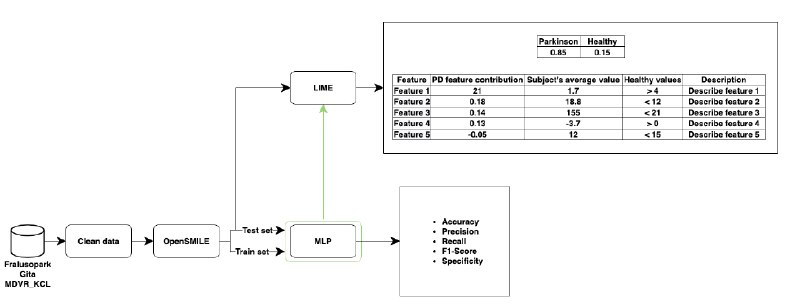
\includegraphics[clip=true, width=\textwidth]{figs/pipeline.png}
	\end{center}
	\caption{Pipeline of the proposed model.}
	\label{pipeline}
\end{figure*}

\pagebreak